% PI-CON architecture — 寬框版。
%
% 設計依據（前幾版的失敗都源於同一個誤判：以為瓶頸是寬度）：
%   真正的瓶頸是「高度」。章首段落後只剩約 10 cm，圖 + caption 必須壓在其內，
%   否則 float 被踢成獨立頁。把框壓窄以求塞進 15 cm 版心，只會讓文字亂折行 →
%   圖反而變高（17.9 x 10.2 cm）→ 踢頁；且每格的字都在跟框邊打架，很醜。
%
% 故反向操作：框加寬到標題一行、描述至多兩行 → 圖矮下來 → 矮了才付得起出血 →
%   出血後 scale ~1，字不縮反漲。目標 19.5 x <= 8.1 cm。
%
% 版面約束（改座標前必讀）：
%   1. update θ 的垂直線必須落在 cfc 的 footprint 內、且在 tf 右緣之外，
%      否則會穿過 Trunk Feature 箱子。cfc 與 tf 不必對齊 x，只要 x 區間錯開即可。
%   2. 箭頭標籤一律折兩行：單行 "Fourier embedding" 需 2.3 cm 間距，兩行只要 1.2 cm。
%   3. inner product 只有 7 個純量（temperature + per-component affine），不佔方塊。
% Compile:  pdflatex architecture_slidestyle_src.tex
\documentclass[tikz, border=2pt]{standalone}
\usepackage{amsmath}
\usetikzlibrary{arrows.meta,positioning,fit,calc}

\definecolor{picon}{HTML}{0072B2}
\definecolor{piconfill}{HTML}{E9F2FB}
\definecolor{inkline}{HTML}{1A1A1A}
\definecolor{incol}{HTML}{009E73}    % Okabe-Ito bluish-green:   輸入
\definecolor{outcol}{HTML}{D55E00}   % Okabe-Ito vermillion:     輸出
\definecolor{traincol}{HTML}{CC79A7} % Okabe-Ito reddish-purple: 訓練迴路

\newcommand{\ttl}[1]{{\large\bfseries #1}}
\newcommand{\btl}[1]{\textcolor{picon}{\large\bfseries #1}}
\newcommand{\sub}[1]{{\normalsize #1}}

\begin{document}%
\hyphenpenalty=10000\exhyphenpenalty=10000\relax
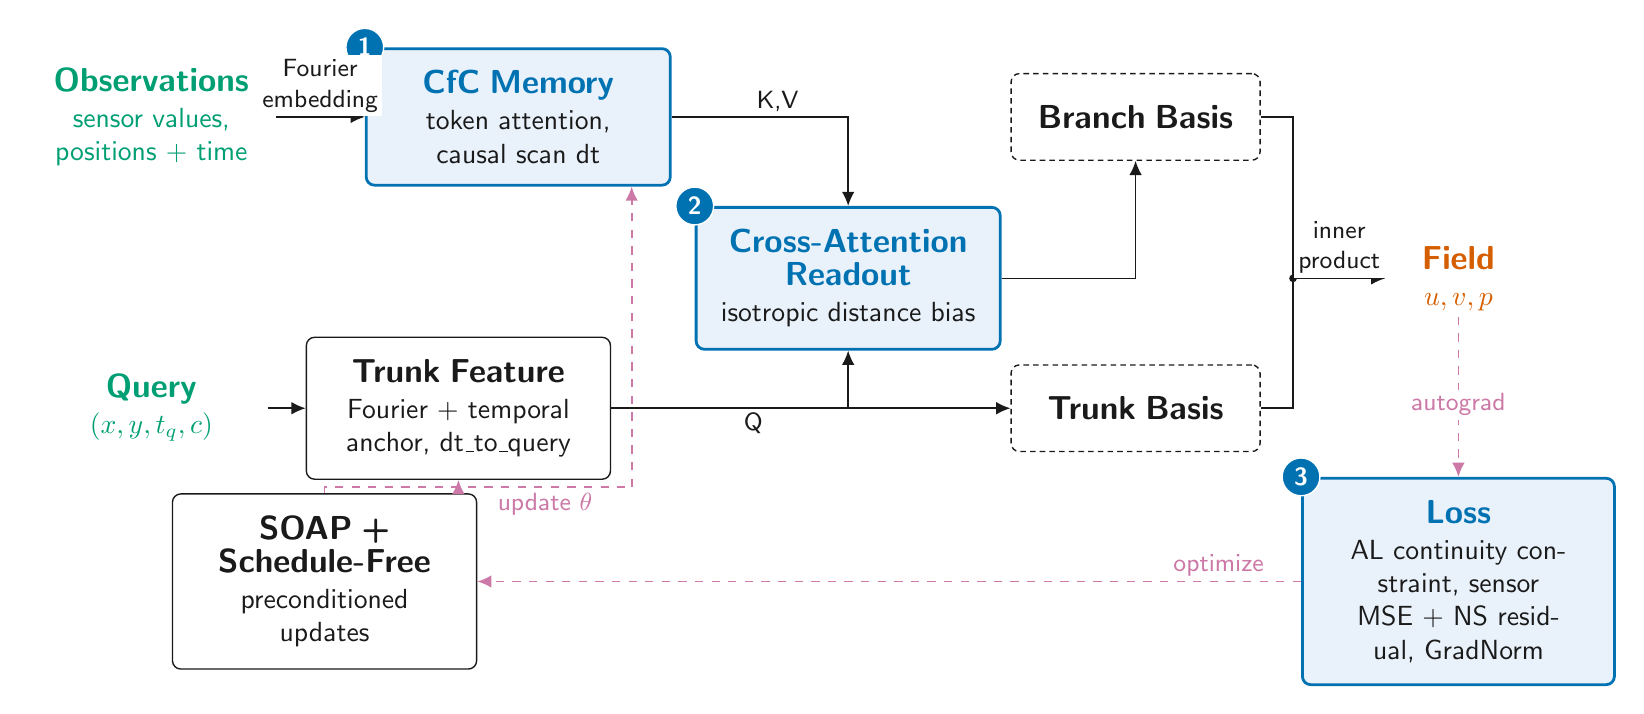
\begin{tikzpicture}[
  font=\sffamily,
  >={Latex[length=1.8mm,width=1.6mm]},
  box/.style={rounded corners=3pt, draw=inkline, line width=0.5pt, fill=white,
              align=center, inner sep=8pt, minimum height=1.1cm, text=inkline},
  % basis：DeepONet 的中間輸出，不是模組 → 虛線框
  basis/.style={rounded corners=3pt, draw=inkline, line width=0.5pt, dash pattern=on 2pt off 1.5pt,
                fill=white, align=center, inner sep=8pt, minimum height=1.1cm, text=inkline},
  picon/.style={rounded corners=3pt, draw=picon, line width=1.0pt, fill=piconfill,
                align=center, inner sep=8pt, minimum height=1.1cm, text=inkline},
  badge/.style={circle, fill=picon, text=white, inner sep=0pt, minimum size=4.8mm,
                font=\sffamily\bfseries\small, draw=white, line width=0.5pt},
  io/.style={align=center, inner sep=2pt},
  arr/.style={->, draw=inkline, line width=0.55pt},
  tarr/.style={->, draw=traincol, line width=0.65pt, dashed},
  tline/.style={draw=traincol, line width=0.65pt, dashed},
  elab/.style={font=\sffamily\small, text=inkline, inner sep=1.5pt, fill=white, align=center},
  tlab/.style={font=\sffamily\small, text=traincol, inner sep=1.5pt, fill=white, align=center},
]

% ---- branch row ----
\node[io,    text width=3.0cm](obs) at (0,0)      {\textcolor{incol}{\ttl{Observations}}\\[1pt]\textcolor{incol}{\sub{sensor values, positions + time}}};
\node[picon, text width=3.3cm](cfc) at (4.66,0)   {\btl{CfC Memory}\\[1pt]\sub{token attention, causal scan dt}};
\node[basis, text width=2.6cm](bb)  at (12.5,0)  {\ttl{Branch Basis}};

% ---- trunk row ----
\node[io,    text width=2.8cm](qry) at (0,-3.7)   {\textcolor{incol}{\ttl{Query}}\\[1pt]\textcolor{incol}{\sub{$(x,y,t_q,c)$}}};
\node[box,   text width=3.3cm](tf)  at (3.9,-3.7) {\ttl{Trunk Feature}\\[1pt]\sub{Fourier + temporal anchor, dt\_to\_query}};
\node[basis, text width=2.6cm](tb)  at (12.5,-3.7){\ttl{Trunk Basis}};

% ---- interaction ----
\node[picon, text width=3.3cm](ca)  at (8.85,-2.05){\btl{Cross-Attention Readout}\\[1pt]\sub{isotropic distance bias}};

% ---- fusion + output ----
\coordinate (mrg) at (14.5,-2.05);
\node[io,    text width=1.7cm](fld) at (16.6,-2.05){\textcolor{outcol}{\ttl{Field}}\\[1pt]\textcolor{outcol}{\sub{$u,v,p$}}};

% ---- 訓練迴路 ----
\node[picon, text width=3.4cm](loss)at (16.6,-5.9){\btl{Loss}\\[1pt]\sub{AL continuity constraint, sensor MSE + NS residual, GradNorm}};
\node[box,   text width=3.3cm](opt) at (2.2,-5.9) {\ttl{SOAP + Schedule-Free}\\[1pt]\sub{preconditioned updates}};

\node[badge] at (cfc.north west)  {1};
\node[badge] at (ca.north west)   {2};
\node[badge] at (loss.north west) {3};

% ---- arrows ----
\draw[arr] (obs) -- (cfc) node[elab, midway, above] {Fourier\\ embedding};
\draw[arr] (qry) -- (tf);
\draw[arr] (cfc.east) -| (ca.north) node[elab, pos=0.3, above] {K,V};
\draw[arr] (tf.east)  -| (ca.south) node[elab, pos=0.3, below] {Q};
\draw[arr] (tf.east) -- (tb.west);
\draw[arr] (ca.east) -| (bb.south);
\draw[draw=inkline, line width=0.55pt] (bb.east) -| (mrg);
\draw[draw=inkline, line width=0.55pt] (tb.east) -| (mrg);
\fill[inkline] (mrg) circle (1.4pt);
\draw[arr] (mrg) -- (fld) node[elab, midway, above] {inner\\ product};

% 訓練迴路（紫）：梯度下行 → optimizer → 參數更新回饋到兩條 path 的可訓練模組。
% cfc 的垂直線走 x=6.1：落在 cfc footprint(2.87..6.45) 內，且在 tf 右緣(5.69) 之外。
\draw[tarr] (fld.south) -- (loss.north) node[tlab, pos=0.55] {autograd};
\draw[tarr] (loss.west) -- (opt.east) node[tlab, pos=0.1, above] {optimize};
\coordinate (cu) at (6.1,-4.7);
\draw[tline] (opt.north) -- (2.2,-4.7) -- (cu);
\node[tlab] at (5.0,-4.92) {update $\theta$};
\draw[tarr] (3.9,-4.7) -- (tf.south);
% x 取 6.1（cfc footprint 內、tf 右緣外），y 取 cfc.south → 垂直而非斜線
\draw[tarr] (cu) -- (cu |- cfc.south);

\end{tikzpicture}%
\end{document}
